%%%%%%%%%%%%%%%%%%%%%%%%%%%%%%%%%%%%%%%%%
% a0poster Landscape Poster
% LaTeX Template
% Version 1.0 (22/06/13)
%
% The a0poster class was created by:
% Gerlinde Kettl and Matthias Weiser (tex@kettl.de)
% 
% This template has been downloaded from:
% http://www.LaTeXTemplates.com
%
% License:
% CC BY-NC-SA 3.0 (http://creativecommons.org/licenses/by-nc-sa/3.0/)
%
%%%%%%%%%%%%%%%%%%%%%%%%%%%%%%%%%%%%%%%%%

%----------------------------------------------------------------------------------------
%	PACKAGES AND OTHER DOCUMENT CONFIGURATIONS
%----------------------------------------------------------------------------------------

\documentclass[a0,landscape]{a0poster}

\usepackage{multicol} % This is so we can have multiple columns of text side-by-side
\columnsep=100pt % This is the amount of white space between the columns in the poster
\columnseprule=3pt % This is the thickness of the black line between the columns in the poster

\usepackage[svgnames]{xcolor} % Specify colors by their 'svgnames', for a full list of all colors available see here: http://www.latextemplates.com/svgnames-colors

\usepackage{times} % Use the times font
%\usepackage{palatino} % Uncomment to use the Palatino font

\usepackage{graphicx} % Required for including images
\graphicspath{{figures/}} % Location of the graphics files
\usepackage{booktabs} % Top and bottom rules for table
\usepackage[font=small,labelfont=bf]{caption} % Required for specifying captions to tables and figures
\usepackage{amsfonts, amsmath, amsthm, amssymb} % For math fonts, symbols and environments
\usepackage{wrapfig} % Allows wrapping text around tables and figures

\begin{document}

%----------------------------------------------------------------------------------------
%	POSTER HEADER 
%----------------------------------------------------------------------------------------

% The header is divided into three boxes:
% The first is 55% wide and houses the title, subtitle, names and university/organization
% The second is 25% wide and houses contact information
% The third is 19% wide and houses a logo for your university/organization or a photo of you
% The widths of these boxes can be easily edited to accommodate your content as you see fit

\begin{minipage}[b]{0.55\linewidth}
\veryHuge \color{NavyBlue} \textbf{ICT and Future Productivity} \color{Black}\\ % Title
\Huge\textit{Evidence and Theory of a GPT}\\[1cm] % Subtitle
\huge \textbf{Marco Brianti \& Laura Gati}\\ % Author(s)
\huge Boston College\\ % University/organization
\end{minipage}
%
\begin{minipage}[b]{0.25\linewidth}
\color{DarkSlateGray}\Large \textbf{Contact Information:}\\
Department of Economics\\ % Address
Boston College\\
140 Commonwealth Avenue, Chestnut Hill, MA \\\\
Phone: +1 (617) 552 3670\\ % Phone number
Email: \texttt{brianti@bc.edu, gati@bc.edu}\\ % Email address
\end{minipage}
%
\begin{minipage}[b]{0.19\linewidth}

\includegraphics[width=25cm]{logo.jpg} % Logo or a photo of you, adjust its dimensions here
\end{minipage}

\vspace{1cm} % A bit of extra whitespace between the header and poster content

%----------------------------------------------------------------------------------------

\begin{multicols}{4} % This is how many columns your poster will be broken into, a poster with many figures may benefit from less columns whereas a text-heavy poster benefits from more

%----------------------------------------------------------------------------------------
%	ABSTRACT
%----------------------------------------------------------------------------------------

\color{Black} % Navy color for the abstract
%\color{Navy} % Navy color for the abstract


%\begin{abstract}

%We employ Structural VARs to investigate the effects of technological shocks specific to the ICT sector on Total Factor Productivity (TFP) and other macroeconomic variables. In response to this sector-specific technological change, relative prices of ICT goods and services immediately fall, ICT investment rises on impact, and TFP displays a significant delayed and persistent increase. Moreover, current ICT supply shocks explain almost one third of overall TFP fluctuations over a 10-year horizon. Taking up the view of theories of ICT as a general-purpose technology, we analyze a two-sector general equilibrium model in order to rationalize previous results and estimate spillovers from the stock of ICT via impulse-response matching. We conclude that ICT accumulation is able to enhance productivity through a positive spillover effect which takes into account the overall level of diffusion of ICT capital in the economy.

%\end{abstract}



%----------------------------------------------------------------------------------------
%	INTRODUCTION
%----------------------------------------------------------------------------------------

%\color{SaddleBrown} % SaddleBrown color for the introduction

\section*{Introduction}

Although there is large consensus on the importance of productivity as a driver of economic performance, there is less agreement on the underlying sources of productivity growth. Along with \cite{comin2006medium}, theoretical contributions rationalize endogenous productivity dynamics by incorporating features of endogenous growth models in standard models of business cycles. Following \cite{romer1990endogenous}, most of these papers augment final-good production functions with an expanding composite of intermediate goods invented by the Research \& Development (R\&D) sector in order to allow for an endogenous rate of adoption of new technologies. Motivated by this wave of research, this paper follows a different path and argues that Information and Communication Technology (hereafter ICT) plays an important role in driving medium-term productivity in sectors that are ICT users.

%----------------------------------------------------------------------------------------
%	OBJECTIVES
%----------------------------------------------------------------------------------------

%\color{DarkSlateGray} % DarkSlateGray color for the rest of the content

\section*{Main Objectives}

\begin{enumerate}
\item Provide robust empirical evidence to show that current rises in ICT investment explain significant and persistent increases in future Total Factor Productivity (hereafter TFP)
\item Analyze a standard theoretical framework in order to both rationalize our empirical results and to draw conclusions concerning the nature of the ICT contribution to future productivity
\end{enumerate}

%----------------------------------------------------------------------------------------
%	MATERIALS AND METHODS
%----------------------------------------------------------------------------------------

\section*{Empirics}

We identify technological shocks specific to the ICT sector in a Structural VAR context. Our multivariate system includes three key variables: TFP, ICT investment (hereafter ICTI), and relative prices (hereafter RP).\footnote{ICTI is defined as the total expenditure in equipment and computer software meant to be used in production for more than a year. Thus, an increase in ICTI is ICT capital deepening. RP is the ratio between the price level of ICT durable goods and the price level in the overall economy.} We use two main identifying restrictions in order to back out an ICT technology shock: (i) it must be orthogonal to current total factor productivity and (ii) maximize the impact effect on ICT investment. Although our results are robust over different specifications, a critique to our empirical strategy is reverse causality coming from news on future TFP. The heart of these robustness checks is sequential identification of news and ICT shocks: we first identify a news shock in the spirit of \cite{barsky2011news}, and subsequently we identify our sectoral ICT shock using the previous identification strategy.

%------------------------------------------------

\subsection*{Identification Strategy}
\subsubsection*{Step 1 - Identification of $\gamma_{news}$}
$$
\max_{\gamma_{news}} \Omega_{1,news}(h) = \frac{ \sum_{t=0}^h e_1' B^t \tilde{A}_0 \gamma_{news} \gamma_{news}' \tilde{A}_0' B'^t e_1 } {e_1' ( \sum_{\tau = 0}^H B^t \Sigma B'^t )e_1}
$$
subject to
$$
\Pi_{1,news}(0) = 0,
$$
$$
\Pi_{6,news}(0) = \Pi_{6,news}(1) = \Pi_{6,news}(2) = 0, \ \ \text{and}
$$
$$
\gamma_{news} \gamma_{news}' = 1.
$$
where the first constraint represents the zero-impact restriction of news on TFP. The second constraint dictates that the response of relative prices to news should be relatively small.\footnote{Our identification strategy is robust to different restrictions to relative prices. Results hold if we set the zero restriction on other horizons.} Finally, the last constraint imposes that $\gamma_{news}$ should be a column derived from an orthogonal matrix. 


\subsubsection*{Step 2 - Identification of $\gamma_{ICT}$}
$$
\max_{\gamma_{ICT}} \Pi_{2,ICT}(0) =  e_2' \tilde{A}_0 \gamma_{ICT} 
$$
subject to
$$
\Pi_{1,ICT}(0) = 0,
$$
$$
\gamma_{news} \gamma_{ICT}' = 0, \ \ \text{and} \ \ \gamma_{ICT} \gamma_{ICT}' = 1.
$$
where the first constraint represents the zero-impact restriction of ICT on TFP and the last constraint imposes that both $\gamma_{news}$ and $\gamma_{ICT}$ should be two different columns derived from an orthogonal matrix.


%----------------------------------------------------------------------------------------
%	RESULTS 
%----------------------------------------------------------------------------------------

\begin{center}\vspace{1cm}
	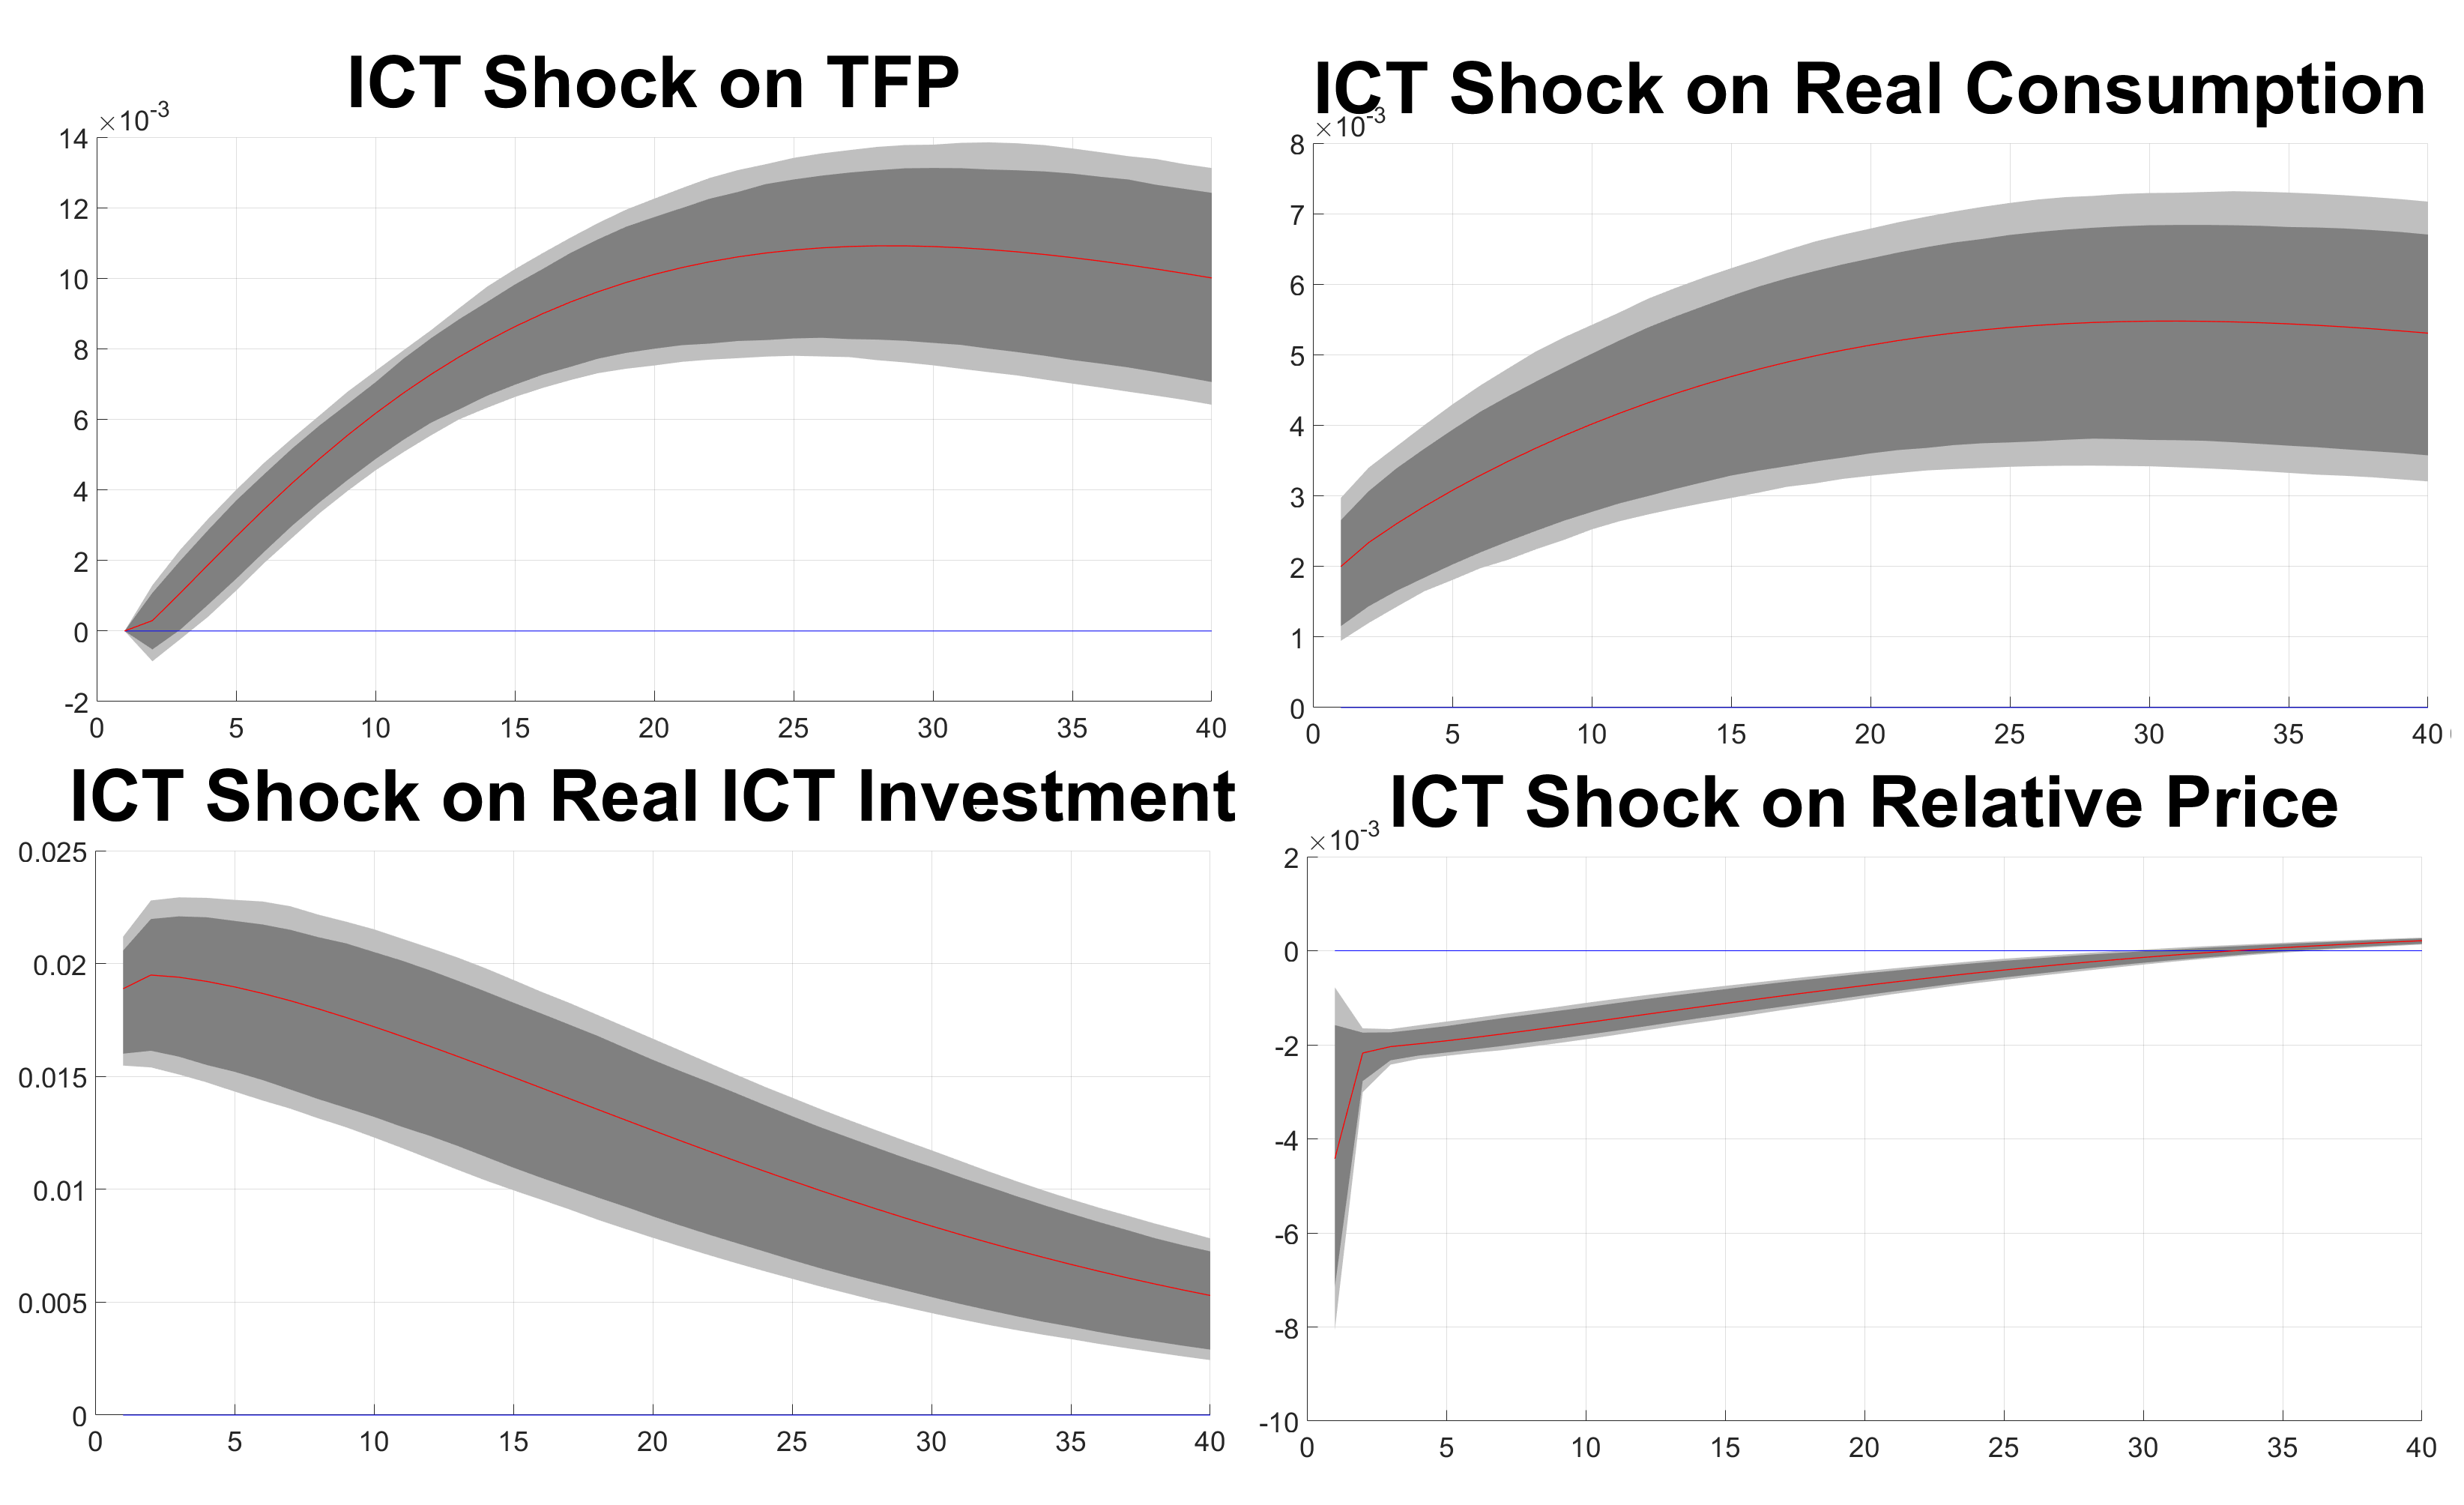
\includegraphics[width=1\linewidth]{alltogether}
	\captionof{figure}{The red solid lines are the estimated impulse responses to our ICT shock. The shaded dark gray area and the shaded light gray area are the $90$\% and $95$\% confidence intervals, respectively, from 2000 bias-corrected bootstrap replications of the reduced-form VAR. The horizontal axes refer to forecast horizon and the units of the vertical axes are percentage deviations.}
\end{center}\vspace{1cm}

\section*{Empirical Results}

In response to the ICT shock, ICTI rises on impact and remains significant for several quarters. RP persistently and significantly declines for more than two years, suggesting that we are indeed identifying the correct sectoral shock. Our main result is that TFP, restricted not to respond on impact, rises after few quarters and remains significant and stable for at least 5 years, despite the tiny size of the ICT sector relative to the economy. Finally, variance decomposition analysis suggests that ICT shocks explain a remarkable size of economic fluctuations over the medium and long run. These shocks drive about $40$\% and $33$\% of the overall GDP and TFP fluctuations over a 10-year horizon, respectively.

\section*{Theory}

In order to understand the economics behind our empirical results, we then analyze a two-sector DSGE model which allows ICT to be the general-purpose technology (hereafter GPT) of the whole economy. In our model, both sectoral production functions are fed with three inputs: (i) labor, supplied by households, (ii) hard capital, produced by the final sector, and (iii) ICT capital, produced by the ICT sector. We then interpret ICT as the GPT of the last 30 years of the U.S. economy assuming that exogenous technological changes in the ICT sector are able to affect economy-wide productivity well above the direct effect coming from the technology increase itself.

\section*{Main Assumption}

Production functions are described as follows
\begin{eqnarray*}
\begin{aligned}
y^c_t(j) &= A^c_t \ \big( k^c_{t}(j) \big)^a \ \big( k^i_{t}(j) \big)^b \ \big( l_{t}(j) \big)^{1-a-b}, \ \ 0 < a,b < 1 \\
y^i_t(q) &= A_t^i \ \big( k^c_{t}(q) \big)^a \ \big( k^i_{t}(q) \big)^b \ \big( l_{t}(q) \big)^{1-a-b}, \ \ 0 < a,b < 1
\end{aligned}
\end{eqnarray*}
where $A_t^c = \eta_t \ \theta^c_t \ (k^i_{t})^{\gamma}$ and $A_t^i = \eta_t \ \theta^i_t \ (k^i_{t})^{\gamma}$.

\begin{center}\vspace{1cm}
	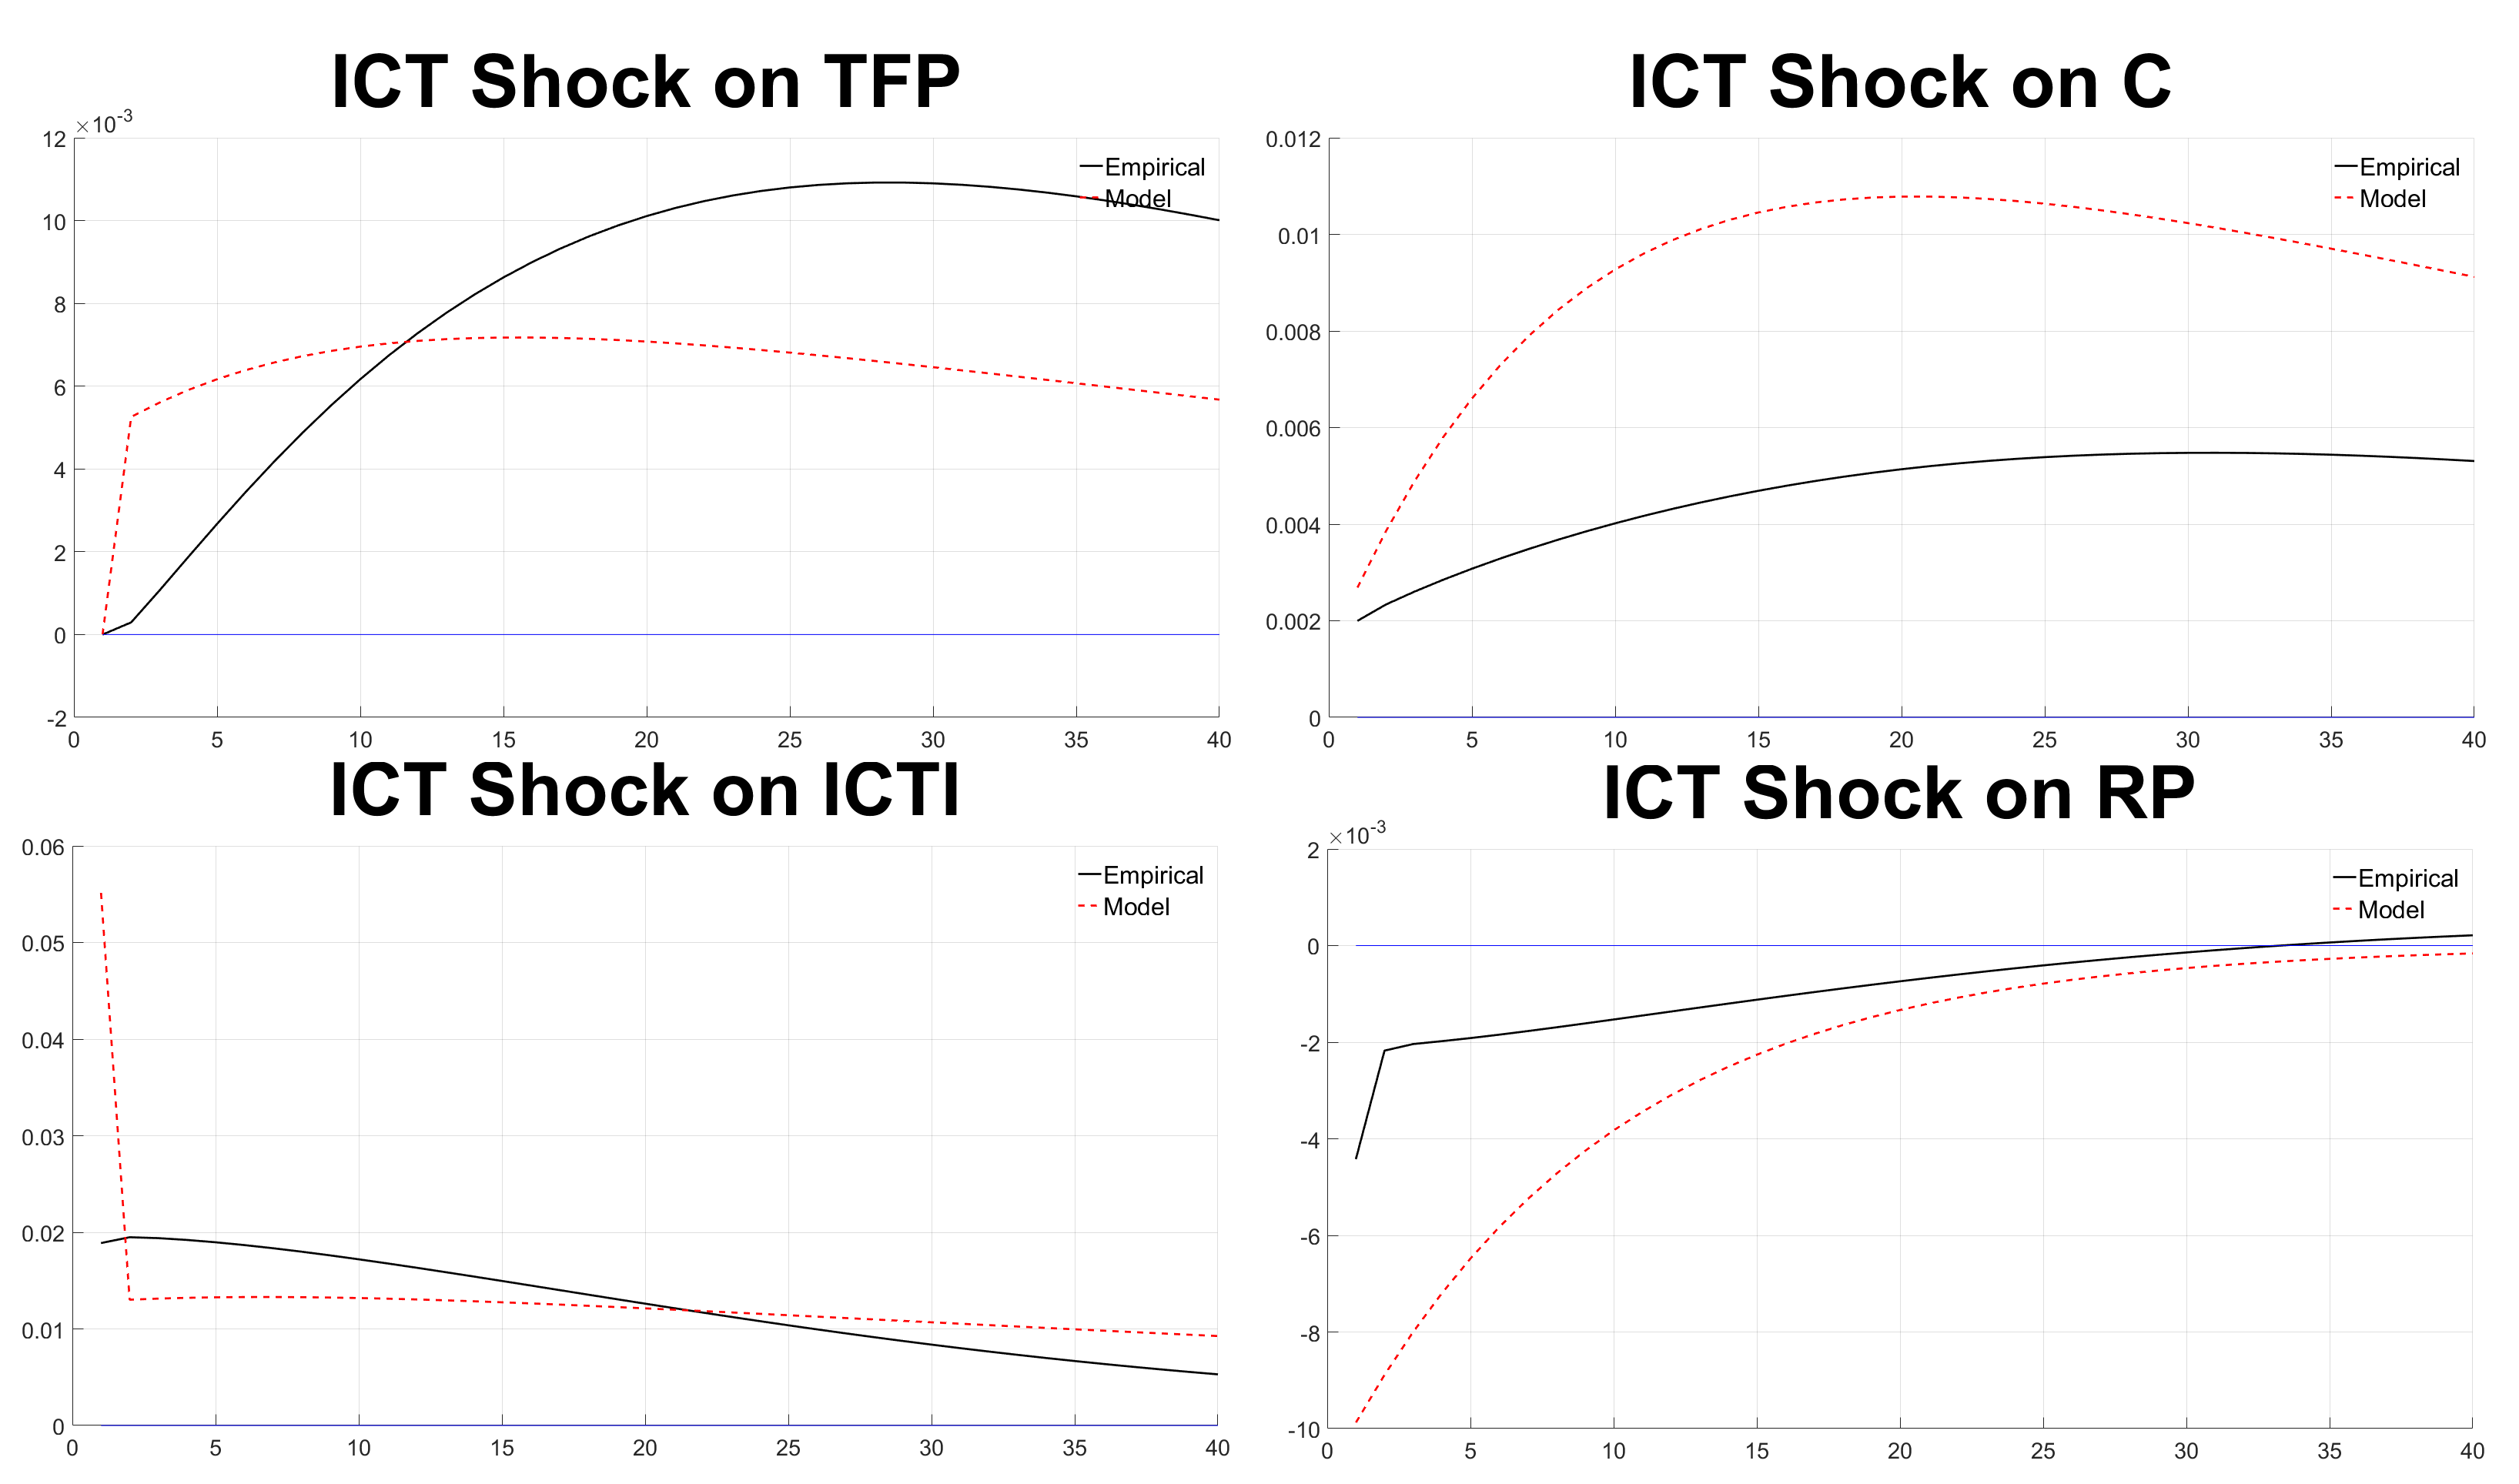
\includegraphics[width=1\linewidth]{IRmatchingall}
	\captionof{figure}{Empirical VAR versus model responses to an ICT shock. The black solid lines show the empirical responses to an identified ICT shock. The dotted red lines show the model’s responses to a shock to the ICT-specific technological component. The horizontal axes refer to forecast horizon and the units of the vertical axes are percentage deviations.}
\end{center}\vspace{1cm}

\section*{Theoretical Results}

The question we tried to answer is why a contemporaneous technological shock specific to the ICT sector is able to trigger increases in future total factor productivity even when it is too small to affect TFP today. When an ICT technology shock hits the economy, both sectors invest more on ICT capital goods since they are now cheaper to purchase and easier to produce. Now, in order to link current higher investment in ICT goods to future TFP, we assume that the general-purpose nature of ICT goods manifests itself in the form of a spillover on both production functions which is not internalized by the agents.\footnote{This externality is governed by the parameter $\gamma$ which has been estimated via impulse-response matching to be robustly larger than zero.} Since the spillover comes from the overall stock of ICT capital, we interpret it as the diffusion of ICT capital.

There is clear economic intuition underlying our assumption of the spillover. Since the purpose of ICT goods is to enhance communication, the quality and speed of information acquisition and sharing is also determined by the overall diffusion of ICT goods. As a simple example, owning a mobile phone enables one to contact another person instantaneously only if the other person is also endowed with the same technology. As a result, the effectiveness of ICT capital is intrinsically related to its own diffusion. The impulse response matching exercise shows that a two-sector model featuring ICT capital and hard capital can successfully match the empirical responses to an ICT shock if the spillover effect is in action. 




%----------------------------------------------------------------------------------------
%	CONCLUSIONS
%----------------------------------------------------------------------------------------

%\color{SaddleBrown} % SaddleBrown color for the conclusions to make them stand out

\section*{Conclusions}

In this project, we look at the effect of ICT shocks on medium-run TFP from both an empirical and a theoretical perspective. In response to an ICT shock TFP rises after three quarters and remains significant for more than 10-years. We rationalize our empirical results by analyzing a two-sector DSGE model \`a la \cite{greenwood1997long}. We use both empirical and theoretical results to estimate main parameters of the model via impulse-response matching to an ICT technology shock. Results show that the parameter which governs the size of the spillover effect is positive and large, suggesting that our interpretation of the general-purpose nature of ICT capital is confirmed by the data.

Thus the main takeaway of this paper is that the interpretation of ICT as a general-purpose technology of the US between 1989-2017 is a good explanation of medium-run TFP growth dynamics. This relies on understanding the general-purpose nature of ICT goods as the extent to which their diffusion in the economy matters. 


%----------------------------------------------------------------------------------------
%	FORTHCOMING RESEARCH
%----------------------------------------------------------------------------------------

\section*{Forthcoming Research}

Augment the model with capital adjustment costs in order to match the slow response displayed by productivity after a ICT shock. 

 %----------------------------------------------------------------------------------------
%	REFERENCES
%----------------------------------------------------------------------------------------

%\nocite{*} % Print all references regardless of whether they were cited in the poster or not
\bibliographystyle{Plain} % Plain referencing style
\bibliography{literature} % Use the example bibliography file sample.bib

%----------------------------------------------------------------------------------------
%	ACKNOWLEDGEMENTS
%----------------------------------------------------------------------------------------

\section*{Acknowledgements}

We thank Professors of Boston College, Department of Economics for the support during the realization of this project.

%----------------------------------------------------------------------------------------

\end{multicols}
\end{document}